\chapter{Implementation, Testing, and Maintenance}
\section{Introduction to Languages}
\begin{figure}[h]
	\centering
\includegraphics[scale=0.8]{images/python_logo.png}
	\caption{Python Logo}
\end{figure}
Python is a dynamic, interpreted (bytecode-compiled) language. There are no type declarations of variables, parameters, functions, or methods in source code. This makes the code short and flexible, and you lose the compile-time type checking of the source code. Python tracks the types of all values at runtime and flags code that does not make sense as it runs.

An excellent way to see how Python code works is to run the Python interpreter and type code right into it.

Python source files use the ".py" extension and are called "modules.". Python is a great and friendly language to use and learn. It fun, and can be adapted to both small and large projects. Python will cut your development time greatly and overall, its much faster to write Python than other languages.

\textbf{Installing} Python is generally easy, and nowadays many Linux and UNIX distributions include a recent Python. Even some Windows computers now come with Python already installed.\\
In order to use Python, it must first be installed on your computer. Follow these steps.
\begin{enumerate}
	\item Go to the python website www.python.org and click on the 'Download' menu choice.
	\item Next click on the Python 3.5 (note the version number may change) Windows Installer to download the installer. If you know you're running a 64-bit os, you can choose the x86-64 installer.
	\item Once you've downloaded the file, open it.
	\item Once the installer starts, it will ask who to install the program for. Usually installing for all users is the best choice.
	\item Next, it needs to know where to install the file. The default choice is fine.
	\item After installed, you should now have a Python menu choice. Start the program by choosing IDLE (Python GUI)
\end{enumerate}

\section{Introduction to IDE’s}
\textbf{{\large IDLE}}\\
IDLE (Integrated DeveLopment Environment or Integrated Development and Learning Environment) is an integrated development environment for Python, which has been bundled with the default implementation of the language since 1.5.2b1.. It is packaged as an optional part of the Python packaging with many Linux distributions. It is completely written in Python and the Tkinter GUI toolkit\\
IDLE has the following features:
\begin{itemize}
	\item coded in 100\% pure Python, using the Tkinter GUI toolkit.
	\item cross-platform: works on Windows and Unix.
	\item multi-window text editor with multiple undo, Python colorizing and many other features, e.g. smart indent and call tips.
	\item Python shell window (a.k.a. interactive interpreter)
	\item debugger (not complete, but you can set breakpoints, view and step)
\end{itemize}
\textbf{{\large PyCharm}}\\
PyCharm is an Integrated Development Environment (IDE) used in computer programming, specifically for the Python language. It is developed by the Czech company JetBrains.

PyCharm provides smart code completion, code inspections, on-the-fly error highlighting and quick-fixes, along with automated code refactorings and rich navigation capabilities.

PyCharm is cross-platform, with Windows, macOS and Linux versions. The Community Edition is released under the Apache License and there is also Professional Edition released under a proprietary license - that has extra features.
\newpage
\noindent PyCharm Features are:-
\begin{itemize}
	\item Intelligent Code Editor\\PyCharm’s smart code editor provides first-class support for Python, JavaScript, CoffeeScript, TypeScript, CSS, popular template languages and more.
	\item Smart Code Navigation\\Use smart search to jump to any class, file or symbol, or even any IDE action or tool window.
	\item Fast and Safe Refactorings\\Refactor the code the intelligent way, with safe Rename and Delete, Extract Method, Introduce Variable, Inline Variable or Method, and other refactorings. Language and framework-specific refactorings helps perform project-wide changes.
	\item VCS, Deployment and Remote Development\\Save time with a unified UI for working with Git, SVN, Mercurial or other version control systems. Run and debug the application on remote machines. Easily configure automatic deployment to a remote host or VM and manage the infrastructure with Vagrant and Docker.
	\item Database tools\\Access Oracle, SQL Server, PostgreSQL, MySQL and other databases right from the IDE. Rely on PyCharm’s help when editing SQL code, running queries, browsing data, and altering schemas.
	\item Python Web frameworks\\PyCharm offers great framework-specific support for modern web development frameworks such as Django, Flask, Google App Engine, Pyramid, and web2py, including Django templates debugger, manage.py and appcfg.py tools, special autocompletion and navigation.
	\item IPython Notebook integration\\PyCharm integrates with IPython Notebook and delivers a solution that combines the advantages of IPython Notebook with extra benefits that the most intelligent Python IDE can offer, including autocompletion, navigation, error checking, etc.
	\item Integrated Unit Testing, with line-by-line code coverage
\end{itemize}
\newpage
\section{Introduction to Tools and Technologies used for Implementation}
\textbf{{\Large TensorFlow}}
\begin{figure}[h]
	\centering
\includegraphics[scale=0.75]{images/tensorflow_logo.png}
	\caption{Tensorflow Logo}
\end{figure}\\TensorFlow is an open source software library for machine learning across a range of tasks, and developed by Google to meet their needs for systems capable of building and training neural networks to detect and decipher patterns and correlations, analogous to the learning and reasoning which humans use.

TensorFlow was originally developed by the Google Brain team for internal Google use before being released under the Apache 2.0 open source license on November 9, 2015.

TensorFlow provides a Python API, as well as C++, Haskell, Java and Go APIs.

\noindent\textbf{Installing TensorFlow on Windows}\\Determine which TensorFlow to install:
\begin{itemize}
	\item \textbf{TensorFlow with CPU support only}. If your system does not have a NVIDIA GPU, you must install this version. Note that this version of TensorFlow is typically much easier to install (typically, in 5 or 10 minutes), so even if you have an NVIDIA GPU, we recommend installing this version first.
	\item \textbf{TensorFlow with GPU support.} TensorFlow programs typically run significantly faster on a GPU than on a CPU. Therefore, if your system has a NVIDIA GPU meeting the prerequisites shown below and you need to run performance-critical applications, you should ultimately install this version.
\end{itemize}
Determine how to install TensorFlow.\\ Pick the mechanism by which you install TensorFlow. The supported choices are as follows:
\begin{itemize}
	\item "native" pip\\Native pip installs TensorFlow directly on your system without going through a virtual environment. Since a native pip installation is not walled-off in a separate container, the pip installation might interfere with other Python-based installations on your system.\\
	To install the CPU-only version of TensorFlow, enter the following command:
	\begin{lstlisting}
pip3 install --upgrade tensorflow
	\end{lstlisting}
	To install the GPU version of TensorFlow, enter the following command:
	\begin{lstlisting}
pip3 install --upgrade tensorflow-gpu
	\end{lstlisting}
	\item Anaconda\\In Anaconda, you may use conda to create a virtual environment. However, within Anaconda, we recommend installing TensorFlow with the pip install command, not with the conda install command.
\end{itemize}
\textbf{{\Large NumPy}}
\begin{figure}[h]
	\centering
\includegraphics[scale=0.75]{images/numpy_logo.jpg}
	\caption{NumPy Logo}
\end{figure}\\NumPy is a library for the Python programming language, adding support for large, multi-dimensional arrays and matrices, along with a large collection of high-level mathematical functions to operate on these arrays.\\
NumPy is the fundamental package for scientific computing with Python. It contains among other things:
\begin{itemize}
	\item A powerful N-dimensional array object.
	\item Sophisticated (broadcasting) functions
	\item Tools for integrating C/C++ and Fortran code
	\item Useful linear algebra, Fourier transform, and random number capabilities
\end{itemize}
\textbf{Installing NumPy via pip}\\
Mac and Linux users can install pre-built binary packages for the SciPy stack using pip. Pip can install pre-built binary packages in the wheel package format.
\begin{lstlisting}
pip install "numpy-1.12.1+mkl-cp35-cp35m-win_amd64.whl"
\end{lstlisting}
\textbf{{\Large TFLearn}}\\TFlearn is a modular and transparent deep learning library built on top of Tensorflow. It was designed to provide a higher-level API to TensorFlow in order to facilitate and speed-up experimentations, while remaining fully transparent and compatible with it.The high-level API currently supports most of recent deep learning models, such as Convolutions, LSTM, BiRNN, BatchNorm, PReLU, Residual networks, Generative networks.\\TFLearn features include:
\begin{itemize}
	\item Easy-to-use and understand high-level API for implementing deep neural networks, with tutorial and examples.
	\item Fast prototyping through highly modular built-in neural network layers, regularizers, optimizers, metrics.
	\item Full transparency over Tensorflow. All functions are built over tensors and can be used independently of TFLearn.
	\item Powerful helper functions to train any TensorFlow graph, with support of multiple inputs, outputs and optimizers.
	\item Easy and beautiful graph visualization, with details about weights, gradients, activations and more.
	\item Effortless device placement for using multiple CPU/GPU.
\end{itemize}
\textbf{{\Large SciPy}}
\begin{figure}[h]
	\centering
\includegraphics[scale=0.75]{images/scipy.png}
	\caption{SciPy Logo}
\end{figure}\\SciPy is an open source Python library used for scientific computing and technical computing.\\SciPy contains modules for optimization, linear algebra, integration, interpolation, special functions, FFT, signal and image processing, ODE solvers and other tasks common in science and engineering.

SciPy builds on the NumPy array object and is part of the NumPy stack which includes tools like Matplotlib, pandas and SymPy. There is an expanding set of scientific computing libraries that are being added to the NumPy stack every day.

\noindent\textbf{Installing SciPy via pip}\\
Mac and Linux users can install pre-built binary packages for the SciPy stack using pip. Pip can install pre-built binary packages in the wheel package format.
\begin{lstlisting}
pip install "scipy-0.19.0-cp35-cp35m-win_amd64.whl"
\end{lstlisting}

\noindent\textbf{OpenCV}\\OpenCV (Open Source Computer Vision) is a library of programming functions mainly aimed at real-time computer vision. OpenCV (Open Source Computer Vision) is a library of programming functions mainly aimed at real-time computer vision. The library is cross-platform and free for use under the open-source BSD license.

\noindent\textbf{Installing OpenCV via pip}\\OpenCV can be install via pip the python package manager. enter the following command:
\begin{lstlisting}
pip install opencv-python
\end{lstlisting}
\noindent\textbf{Installing OpenCV from prebuilt binaries}
\begin{enumerate}
	\item Below Python packages are to be downloaded and installed to their default locations.
	\begin{enumerate}
		\item Python-2.7.x.
		\item Numpy.
		\item Matplotlib.
	\end{enumerate}
	\item Install all packages into their default locations.
	\item After installation, open Python IDLE. Enter import numpy and make sure Numpy is working fine.
	\item Download latest OpenCV release from sourceforge site and double-click to extract it.
	\item Goto opencv/build/python/2.7 folder.
	\item Copy cv2.pyd to C:/Python27/lib/site-packages.
	\item Open Python IDLE and type following codes in Python terminal.
	\begin{lstlisting}
import cv2
print cv2.__version__
	\end{lstlisting}
\end{enumerate}
If the results are printed out without any errors, You have installed OpenCV-Python successfully.
\pagebreak

\noindent\textbf{GitHub}
\begin{figure}[h]
	\centering
\includegraphics[scale=0.40]{images/github_logo.png}
	\caption{GitHub Logo}
\end{figure}\\GitHub is a Git repository web-based hosting service which offers all of the functionality of Git as well as adding many of its own features. Unlike Git which is strictly a command-line tool, Github provides a web-based graphical interface and desktop as well as mobile integration. It also provides access control and several collaboration features such as wikis, task management, and bug tracking and feature requests for every project.\\
This means that you can do things like:
\begin{itemize}
	\item Frictionless Context Switching.\\ Create a branch to try out an
	idea, commit a few times, switch back to where you branched from,
	apply a patch, switch back to where you are experimenting, and merge
	it in.
	\item Role-Based Code lines. \\ Have a branch that always contains only
	what goes to production, another that you merge work into for testing,
	and several smaller ones for day to day work.
	\item Feature Based Work flow. \\ Create new branches for each new
	feature you're working on so you can seamlessly switch back and forth
	between them, then delete each branch when that feature gets merged
	into your main line.
	\item Disposable Experimentation.\\  Create a branch to experiment in,
	realize it's not going to work, and just delete it - abandoning the
	work—with nobody else ever seeing it (even if you've pushed other
	branches in the meantime).
\end{itemize}
Notably, when you push to a remote repository, you do not have to push
all of your branches. You can choose to share just one of your
branches, a few of them, or all of them. This tends to free people to
try new ideas without worrying about having to plan how and when they
are going to merge it in or share it with others.
\pagebreak

\noindent\textbf{Git}
\begin{figure}[h]
	\centering
\includegraphics[scale=0.30]{images/git_logo.png}
	\caption{Git Logo}
\end{figure}\\Git is a distributed revision control and source code management (SCM) system with an emphasis on speed, data integrity, and support for distributed, non-linear workflows. Git was initially designed and developed by Linus Torvalds for Linux kernel development in 2005, and has since become the most widely adopted version control system for software development.\\

As with most other distributed revision control systems, and unlike most client–server systems, every Git working directory is a full-fledged repository with complete history and full version-tracking capabilities, independent of network access or a central server. Like the Linux kernel, Git is free and open source software distributed under the terms of the GNU General Public License version 2 to handle everything from small to very large projects with speed and efficiency.

\section{Coding Standards}
Python uses indentation to give you a visual indication of the structure of your code. Additionally we have an interactive interpreter which provides a default representation for many objects and data structures. Consistency of style, and using the interpreters representation for objects, will make it easier for you to parse and absorb the meaning of the code.\\
Following are some of the python coding standards adopted during the project:
\begin{itemize}
	\item Python uses 4 spaces per indentation level.
	\item Spaces are the preferred indentation method.
	\item Limit all lines to a maximum of 79 characters.
	\item One statement per line.\\
	While some compound statements such as list comprehensions are allowed and appreciated for their brevity and their expressiveness, it is bad practice to have two disjointed statements on the same line of code.
	\item Continuation lines should align wrapped elements either vertically using Python's implicit line joining inside parentheses, brackets and braces, or using a hanging indent.
	\item Imports should usually be on separate lines.
	\begin{lstlisting}
Ok:
import os
import sys

Not Ok:
import sys, os
	\end{lstlisting}
	\item Imports should be grouped in the following order:
	
	\begin{enumerate}
		\item standard library imports
		\item related third party imports
		\item local application/library specific imports
	\end{enumerate}
	We should put a blank line between each group of imports.
\end{itemize}
\pagebreak

\section{Project Scheduling}
\begin{figure}[h]
	\centering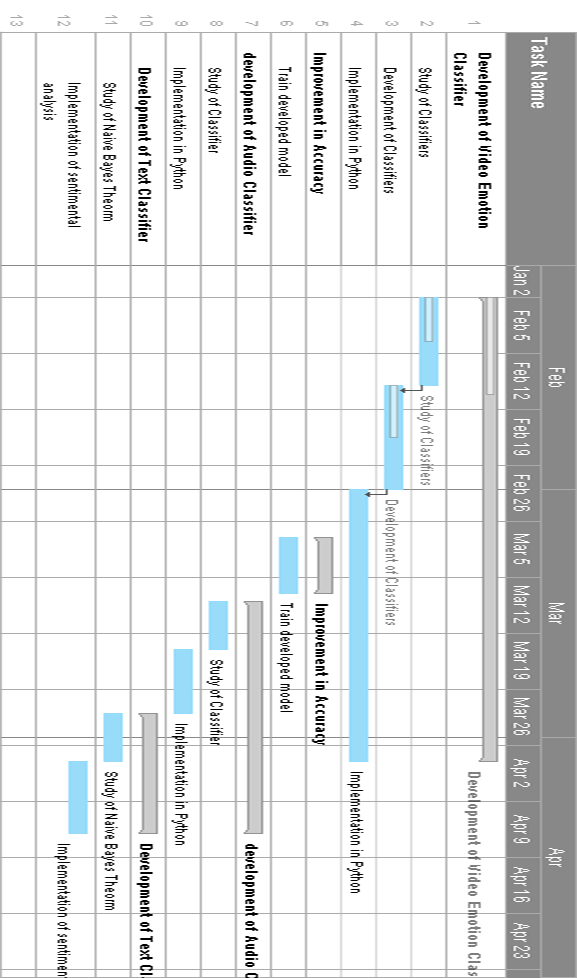
\includegraphics[scale=0.55]{images/gantt_rotate.png}
	\caption{Gantt Chart}
\end{figure}

\section{Testing}
The networks are programmed with use of the TFLearn library on top of TensorFlow, running on Python. This environment lowers the complexity of the code, since only the neuron layers have to be created, instead of every neuron. The program also provides real-time feedback on training progress and accuracy, and makes it easy to save and reuse the model after training.
\begin{enumerate}[(A)]
	\item  The first network to test is based on the previously described research by Krizhevsky and Hinton.This is the smallest network of the three, which means that it has the lowest computational demands. Since one of the future applications might be in the form of live emotion recognition in embedded systems, fast working algorithms are beneficial\\
	The network consists of three convolutional layers and two fully connected layers, combined with maxpooling layers for reducing the image size and a dropout layer to reduce the chance of over fitting. The hyper parameters are chosen such that the number of calculations in each convolutional layer remains roughly the same. This ensures that information is preserved throughout the network. Training is performed using different numbers of convolutional filters to evaluate their effect on the performance.
	\item In 2012, the AlexNet convolutional network was developed for classifying images in more than 1000 different classes, using 1.2 million sample pictures from the ImageNet dataset. Due to the fact that in this research the model only has to distinguish seven emotions, and due to our limited computing resources, the size of the original network is considered to be too large.\\
	Hence, instead of 5 convolutional layers we applied 3, and in the subsequent 3 fully connected layers the number of nodes of each fully connected was reduced from 4096 to 1024. While the original network was divided for parallel training, it was observed that was not necessary for the smaller version. The network also makes use of local normalization to speed up the training and dropout layers in order to reduce the over-fitting
	\item  The last experiments are performed on a network based by the work of Gudi. Since this research also aimed on recognizing 7 emotions using the FERC-2013 dataset, the architecture should be a good starting point for our research.
	The original network starts with an input layer of 48 by 48, matching the size of the input data. This layer is followed by one convolutional layer, a local contrast normalization layer, and a maxpooling layer respectively. The network is finished with two more convolutional layers and one fully connected layer, connected to a softmax output layer. Dropout was applied to the fully connected layer and all layer contain ReLu units.\\
	For our research, a second maxpooling layer is applied to reduce the number of parameters. This lowers the computational intensity of the network, while the reduction in performance is claimed to be only 1-2\%. Furthermore the learning rate is adjusted. Instead of linearly decreasing the learning rate as done by Gudi, we believe a learning rate which makes use of momentum would converge faster, as the momentum increases the learning rate when the gradient keeps going in the same direction.
\end{enumerate}

All networks are trained for 60 epochs with the data of FER2013.
\begin{figure}[h]
	\centering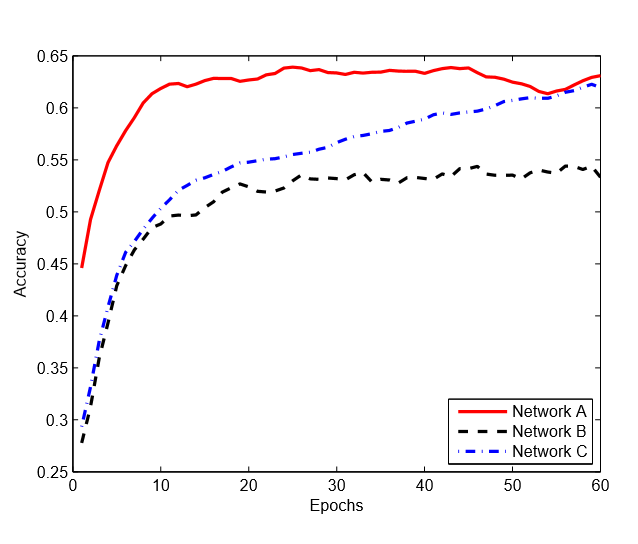
\includegraphics[scale=0.5]{images/training_validation.png}
	\caption{Accuracy on the validation set during training epochs}
\end{figure}

\begin{table}
	\centering
	\caption{Details of the trained networks}
	\begin{tabular}{| c | c | c | c |}
		\hline
		Network & \multicolumn{2}{c |}{Accuracy} & Size\\
		\hline
		& Validation & RaFD &\\
		\hline
		A & 63\% & 50\% & Small\\
		\hline
		B & 53\% & 46\% & Large\\
		\hline
		C & 63\% & 60\% & Medium\\
		\hline
	\end{tabular}
\end{table}
Above figure and table show various details of the training process and the final model. For network A, the final accuracy on the validation data is around 63\%. Already after 10 epochs, the accuracy raised above 60\%, indicating quick learning capabilities. Furthermore it is noteworthy that adjusting the filter dimension did not have a big influence on the accuracy, though it has on the processing time. This means that fast models can be made with very reasonable performance.

Network C shows a somewhat slower learning curve, but the final accuracy on the validation set is similar to that of network A. The processing demands are in between that of the other networks, so based on this fact, network A seems to be the most promising approach for our emotion recognition task. However, the performance of network C on the extra RaFD test-set is significantly better (60\%) than that of network A (50\%).

As can be seen from figure 4.7, the accuracy seems to still increase in the last epochs. We therefore will train the network for 100 epochs in the final run, to make sure the accuracy converges to the optimum.

\begin{figure}[h]
	\centering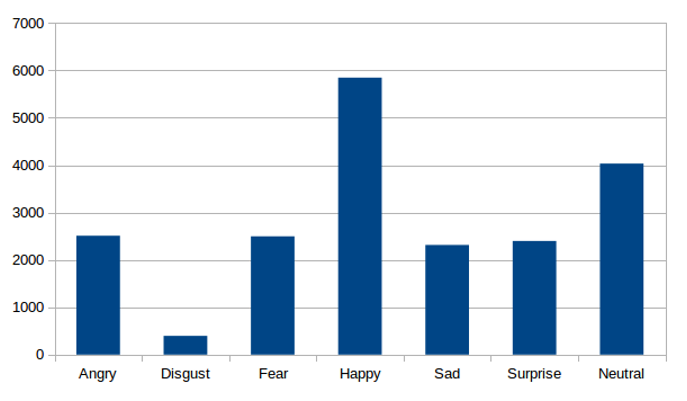
\includegraphics[scale=0.75]{images/images_per_emotion.png}
	\caption{Number of images per emotion in the final training set}
\end{figure}
In an attempt to improve the final model even more, the network will be trained on a larger set than the one described previously. Instead of 9000 pictures, training will be done with 20000 pictures from the FERC2013 dataset. The ratios of the emotions present in this set are given in figure 4.8. Newly composed validation (2000 images) and test sets (1000 images) from the FERC-2013 dataset are used as well, together with the well-balanced RaFD test set from the previous experiment.

The accuracy rates of the final model are given in table 4.2. On all validation and test sets the accuracy was higher than during previous runs, underlining that more data and longer training can improve the performance of a network

\begin{table}[h]
	\centering
	\caption{Accuracy of the networks}
	\begin{tabular}{| c | c | c | c |}
		\hline
		Network & \multicolumn{2}{c |}{FERC-2013} & RaFD\\
		\hline
		& Validation & Test &\\
		\hline
		A & 63\% & & 50\%\\
		\hline
		B & 53\% & & 46\%\\
		\hline
		C & 63\% & & 60\%\\
		\hline
		Final & 66\% & 63\% & 71\%\\
		\hline
	\end{tabular}
\end{table}

 Given that the state-of-the art networks from previous research obtained about 67\% on test sets, and keeping in mind our limited resources, the results are in fact pretty good. Notable is the accuracy on the RaFD test set, which contains completely different pictures than the training data. This illustrates the powerful generalizing capabilities of this final model.
